\documentclass{deliverablereport}
\usepackage[style=alphabetic,backend=bibtex]{biblatex}
\addbibresource{../../lib/kbibs/kwarcpubs.bib}
\addbibresource{../../lib/kbibs/extpubs.bib}
\addbibresource{../../lib/kbibs/kwarccrossrefs.bib}
\addbibresource{../../lib/kbibs/extcrossrefs.bib}
\addbibresource{../../lib/deliverables.bib}
\addbibresource{local.bib}
%\usepackage{local}
\usepackage[hide]{ed}
\usepackage{stex-logo}
\usepackage{rotating}
\usepackage{tikzinput}
\usetikzlibrary{fit}
\title{Curated Math-in-the-Middle Ontology and Alignments for GAP/SAGE/LMFDB}
\def\shorttitle{Curated MitM Ontology/Alignments}

\deliverable{dksbases}{lfmverif}
\deliverydate{4/09/2018}
\duedate{1/09/2018}

\author{John Cremona, Dennis M\"uller, Michael Kohlhase, Markus Pfeiffer, Florian Rabe, Nicolas M. Thiéry, Tom Wiesing}

\begin{document}
\maketitle

\bigskip

\begin{abstract}  Work Package WP6 develops a novel, foundational, knowledge-based framework for
  interfacing existing open source mathematical software systems and knowledge bases into
  a mathematical VRE, where systems can delegate functionalities among each other
  seamlessly without losing semantics.

  The overall Math-in-the-Middle (MitM) Framework developed in WP6 over the last three
  years is described in D6.5; this Report complements it by describing the curated
  contents Math-in-the-Middle (MitM) Ontology which serves as a reference and pivotal
  point for translations between the various input languages of mathematical software
  systems and knowledge bases.

  In a nutshell, the MitM Ontology describes the mathematical objects, concepts, and their
  relations in a general, system-agnostic way in an OMDoc/MMT theory graph while the
  mathematical systems export API theories that describe the system interface language in
  terms of types, classes, constructors, and functions -- again in OMDoc/MMT. These two
  levels of descriptions are linked by OMDoc/MMT alignments that allow the translation of
  expressions between systems.

%%% Local Variables:
%%% mode: visual-line
%%% fill-column: 5000
%%% mode: latex 
%%% TeX-master: "report"
%%% End:
\end{abstract}
%\newpage\strut\githubissuedescription
\newpage\tableofcontents\newpage

\section{Introduction}\label{sec:intro}
\section{Introduction}\label{sec:intro}

\begin{newpart}{MK: adapted from Tom's Thesis}
There is a large and vibrant ecosystem of open-source mathematical software systems.
These systems can range from calculators, which are only capable of performing simple
computations, via mathematical databases (curating collections of a mathematical objects)
to powerful modeling tools and computer algebra systems (CAS). 

Most of these systems are very specific -- they focus on one or very few aspects of
mathematics.  For example, the ``Online Encyclopedia of Integer Sequences''
(OEIS~\cite{Sloane:oeis12,oeis}) focuses on sequences over $\mathbb{Z}$ an their
properties and the ``L-Functions and Modular Forms Database''
(LMFDB)~\cite{Cremona:LMFDB16,lmfdb:on} objects in number theory pertaining to Langland's
program.  GAP~\cite{GAP:on} excels at discrete algebra, whereas
SageMath~\cite{SageMath:on} focuses on Algebra and Geometry in general, and
Singular~\cite{singular:on} on polynomial computations, with special emphasis on
commutative and non-commutative algebra, algebraic geometry, and singularity theory.

For a mathematician however (a user; let us call her Jane) the systems themselves are not relevant, instead she only cares about being able to solve problems. 
Typically, it is not possible to solve a mathematical problem using only a single program. 
Thus Jane needs to work with multiple systems and combine the results to reach a solution. 
Currently there is very little help with this practice, so Jane has to isolate sub-problems the respective systems are amenable to, formulate them into the respective input language, collect results, and reformulate them for the next system a tedious and error-prone process at best, a significant impediment to scientific progress in its overall effect. 
Solutions for some situations certainly exist, which can help get Jane unstuck, but these are ad-hoc and for specific, often-used system combinations only. 
Each of these requires a lot of maintenance and does not scale to a larger set of specialist systems. 

The OpenDreamKit project, which aims at a mathematical VRE toolkit, proposes the Math-in-the-Middle (MitM~\cite{DehKohKon:iop16}) Paradigm, an interoperability framework based on a flexiformal
representation of mathematical knowledge and aligns this with system-generated interface
theories. 

In this paper we instantiate the MitM paradigm with a concrete domain development and
evaluate it on a distributed computing GAP, SageMath and Singular.\ednote{ we generally we
  want to show that the promises in the CICM paper become reality.}

We will use the following example as a running example: Jane wants to act on singular
polynomials with GAP permutation groups\ednote{MK@(MP|VA): }

 \ednote{MK: continue with the structure} 
\end{newpart}

%%% Local Variables:
%%% mode: latex
%%% TeX-master: "paper"
%%% End:
\newpage

\section{The MitM Ontology}\label{sec:mitmonto}
%% types
\newcommand{\fold}[2]{\let\@tmpop=\relax\@for\@I:=#2\do{\@tmpop\@I\let\@tmpop=#1}}
\newcommand{\record}[1]{\{\fold{,}{#1}\}}
\newcommand{\union}[1]{[\fold{,}{#1}]}
\newcommand{\sq}{\subseteq}

In this section, we describe the parts of the MitM ontology, which is a formal development in the MMT system.
The formalizations can be found at \url{https://gl.mathhub.info/MitM/}.
That location also contains various other archives in the \href{https://gl.mathhub.info/MitM/}{\texttt{MitM} library}, which are experiments, where the MitM ontology has been picked up by other projects.

The MitM ontology consists of two parts: the \textbf{MitM Foundation} which provides the logical language in which the mathematical domains in the MitM ontology can be described, and the \textbf{MitM Core}, which consists of the knowledge about these domains represented in the MitM foundation.

\subsection{The MitM Foundation}\label{sec:foundation}

The MitM foundation provides the type system and logic for the MitM ontology, i.e., the basic representational infrastructure used in the MitM ontology.
It is developed in the archive  \href{https://gl.mathhub.info/MitM/Foundation}{\texttt{Foundation}} (4 files, 539 LoF (lines
of formalization), 103 commits).

\paragraph{Types \& Expressions}
While the logic is relatively straightforward, the standardization of the type system was very difficult because mathematics requires a rich, open-ended type system, yet concrete implementations must stay as simple as possible.
After surveying the OpenDreamKit systems, we developed the types described in Appendix~\ref{app:types}.
These types come with a set of constructors that allow to specify expressions (members of the respective type) that represent mathematical objects systematically; see Appendix~\ref{app:expr} for an exemplary list of mathematical objects that can be represented as a members of these types.

In a nutshell, the MitM foundation provides base types for all arithmetical number systems and common data structures like strings/words and Boolean values.
Complex types build on this include structural ones like (total and partial dependent) function, product, record, types, and mathematical constructions like sets, multisets, ists, vectors, and matrices.
In particular, dependent record types allow to represent types for mathematical structures (e.g. rings, fields, polynomials, finite maps, etc.) and their models.
These can also be constructed from OMDoc/MMT theories via the novel \textsf{Mod} operator~\cite{MueRabKoh:tat18}.

Finally, the MtiM foundation supports subtyping for the arithmetical number systems ($\mathbb{N}\subseteq\mathbb{Z}\subseteq\mathbb{Q}\subseteq\mathbb{R}\subseteq\mathbb{C}$), and along the sub-model relation.
This allows to express many mathematical identies very naturally.


% % % % % % % % % % % % % % % % % % % % % % % % % % % % %
\subsection{MitM Core}

The \textbf{MitM core} in the \href{https://gl.mathhub.info/MitM/smglom}{\texttt{smglom}}\footnote{The name \texttt{smglom} was initially chosen for the ``Semantic Multilingual Glossary of Mathematics'' (SMGloM; see \ref{sec:smglom} below) with which it is cross-referenced. We will rethink naming once the MitM Ontology stabilizes.}  archive (55 files, 2600 LoF, 360 commits).
It carries the bulk of the knowledge representation in the MitM Ontology.
The main thrust of curation has been to get the VRE use cases reported on in~\cite{ODK-D6.5}, but we also have elementary formalizations of algebra, arithmetics, calculus, category theory, set collections, elliptic curves (for LMFDB), functional analysis, geometry, graph theory, measure theory, set theory, and topology.

In the sequel, we describe two exemplary parts of the MitM core ontology.

\subsubsection{Computational Group Theory}
Our formalization of CGT (part of the core ontology, found in \texttt{algebra/computational\_groups}) follows the template of its implementation in \GAP, and requires several levels of abstraction -- currently \emph{abstract}, \emph{representation}, \emph{implementation}, and \emph{concrete}. From our experience, we expect this pattern to be applicable across computational algebra, possibly with additional levels of abstraction. 
The left box in Figure \ref{fig:cgtontology} gives an overview.

The abstract level contains the axioms and basic definitions of the theory of \emph{Groups}: generating sets, homomorphisms, group actions, stabilisers, and orbits.
The most basic part is given in Figure~\ref{fig:mitm1}. 
\begin{figure}[ht]\centering
  \fbox{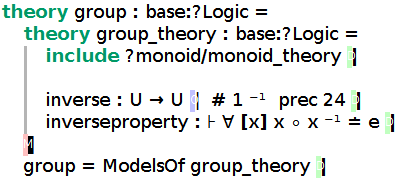
\includegraphics[width=8cm]{../MACIS17-interop/mitm1}}
  \caption{A Formalization of a Group}\label{fig:mitm1}
\end{figure}

At the representation level groups are described as concrete objects
suitable for computations: groups of permutations, groups of matrices,
finitely presented groups, groups obtained by algebraic constructions or using
polycyclic presentations.

At the implementation level, we encode implementation details: for
example, permutation groups are considered as finite subgroups of the group $S_{\mathbb{N}+}$, and defined \ednote{constructed?} by
providing a set of generating permutations.

At the concrete level, the computation happens: while the higher levels
are suitable for mathematical deduction and inference, this level is where OpenDreamKit systems like \GAP perform their main work.

\subsubsection{Modeling and Simulation}

The \href{https://gl.mathhub.info/MitM/smglom}{\texttt{models}}
archive (11 files, 650 LoF, 113 commits) is an experimental extension
of the MitM ontology, where we test the expressive power of MitM
framework (and the OpenDreamKit technologies) by applying it to a
field well outside of mathematics, namely for modeling and simulation
in opto-electronics.

\subsection{The ``Semantic Multilingual Glossary of Mathematics'' (SMGloM)}\label{sec:smglom}

The SMGloM library is available at \url{https://gl.mathhub.info/smglom}. It contains
ca. 815 glossary modules (OMDoc/MMT theories) with more than 1700 concepts. All
represented in \sTeX, a semantic variant of {\LaTeX} developed by FAU and (earlier at)
JacU. Figure~\ref{fig:conductor} shows an example. The boldface words are \emph{definienda}
(i.e. concepts to be defined; here ``conductor'') and the blue ones are concepts already
defined in other parts of the MitM Ontology. SMGloM definitions are multilingual -- mostly
English and German, but also some Romanian, Turkish, Arabic, and Chinese, and are
cross-linked on the concept level.

\ednote{specify what part of it was implemented in and out of \ODK}

\begin{figure}[ht]\centering
  \fbox{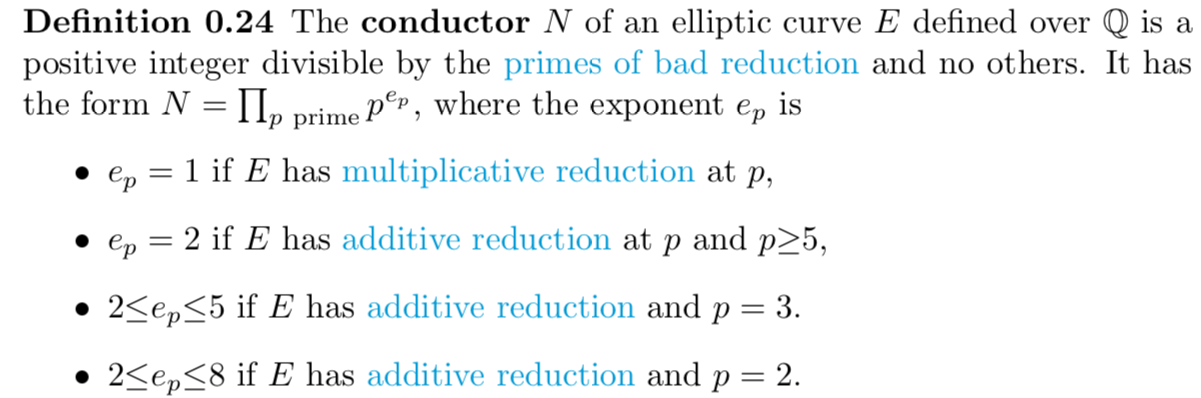
\includegraphics[width=14cm]{conductor}}
  \caption{An \sTeX Definition of the Conductor of an Elliptic
    Curve}\label{fig:conductor}
\end{figure}


%%% Local Variables:
%%% mode: visual-line
%%% fill-column: 5000
%%% mode: latex
%%% TeX-master: "report"
%%% End:

%  LocalWords:  formalizations texttt formalization standardization subsubsection textbf newcommand subseteq textsf MueRabKoh:tat18
%  LocalWords:  compactitem ednote adic ldots,a_n ldots,a_n ldots,T_n ldots Vec monoid sq
%  LocalWords:  FiniteHybridset subtyping emph leq_T leq_ leq_ leq_ r,x s,y leq doteq_T
%  LocalWords:  t,t forall subformula u,p ldots,x cdot cdot Qsqrt Qzeta th smglom fbox
%  LocalWords:  stabilizes fig:cgtontology fig:mitm1 centering includegraphics mathbb
\newpage

\section{The OpenDreamKit System APIs}\label{sec:sysapis}
\subsection{Generated System API Theories}\label{sec:sysapis:gentheories}

We have generated and cross-linked system API theories for the computer algebra systems
GAP, SageMath, and SINGUALAR, as well as the mathematical knowledge base LMFDB. They are
generated from pre-existing sources in the systems like type information, code
annotations, and systematic API documentation.  OpenDreamKit deliverable report, Section
5 of \textbf{D6.5}~\cite{ODK-D6.5} has the details.  


The OpenDreamKit System API Theories can be found at
\url{https://gl.mathhub.info/ODK/{GAP,SAGE,SINGULAR,LMFDB,knowls}}. These contain:
\begin{itemize}
\item \texttt{GAP}: (210 Theories, 8470 Symbols, 64 Commits) \footnote{Since the generated
    API theories do not come from \texttt{.mmt} source files, numbers of files and LoF are
    not informative metrics. Approximately, one \texttt{.mmt} file contains on average
    2--3 theories, and 1--2 LoF correspond to one symbol.}  Generated from a JSON export
  from the GAP system. A theory corresponds to a source file of a GAP package, a symbol
  represents a GAP method or operation.
\item \texttt{Sage}: (5431 Theories, 7279 Symbols, 73 Commits) Analogously generated from
  a JSON export. Theories correspond to Sage categories, symbols to methods.
\item \texttt{Singular}: (179 Theories, 4519 Constants, 6 Commits) \ednote{find out what
    theories represent?}
\item \texttt{LMFDB}: (161 Commits) Consists of schema theories for LMFDB databases
  (currently 5 databases covered, 182LoF) and interface theories for non-mathematical or
  LMFDB-specific concepts (labels, descriptors) represented therein (3 Files, 123 LoF)
\item \texttt{knowls}: (945 flexiformal Theories, ca. 900 Symbols; 10 Commits) generated
  from the LMFDB knowls system of interface documentations. The knowls resource is
  actively maintained and currently under intense review by the LMFDB community. 
\end{itemize}

\subsection{The MitM Alignments}

The MitM alignments are available from \url{https://gl.mathhub.info/alignments/Public} (6
files, 1040 LoF, 240 Commits). They are represented as text files containing pairs of MMT
URIs annotated with various semantic classification schemata;
see~\cite{MueGauKal:cacfms17} for details.\ednote{MK: what else can we write about them?}
\ednote{this figure does not fit in the text width}
\begin{figure}[ht]\centering
  \tikzinput[width=.98\textwidth]{../D6.5/alignmentimg}
  \caption{Alignments between the MitM Ontology and the \GAP API}\label{fig:cgtontology}
\end{figure}

As an example, Figure~\ref{fig:cgtontology} sketches the alignments between the
computational group theory ontology from above and the constructors and operations of
\GAP.

%%% Local Variables:
%%% mode: visual-line
%%% fill-column: 5000
%%% mode: latex
%%% TeX-master: "report"
%%% End:

%  LocalWords:  textbf texttt ednote knowls flexiformal MueGauKal:cacfms17 centering
%  LocalWords:  tikzinput textwidth fig:cgtontology
\newpage

\section{Evaluation \& Conclusion}\label{sec:concl}
\section{Conclusion}\label{sec:concl}

We have shown how to extend the Math-in-the-Middle framework for integrating systems to mathematical data bases like the \lmfdb. 
The main idea is to embed knowledge sources as virtual theories, i.e. theories that are not -- theoretically or in practice -- limited in the number of declarations and allow dynamic loading and processing. 
For accessing real-world knowledge sources, we have developed the notion of codecs and integrated them into the MitM ontology framework. 
These codec's (and their MitM types) lift knowledge source access to the MitM level and thus enable object-level interoperability and allow humans (mathematicians) access using the concepts they are familiar with. 
Finally, we have shown a prototypical query translation facility that allows to delegate some of the processing to the underlying knowledge source and thus avoid thrashing of virtual theories. 

\paragraph{Related Work} Most other integration schemes employ a \textbf{homogenous approach}, where there is a master sytsem and all data is converted into that system. 
A paradigmatic example of this is the Wolfram Language and the Wolfram Alpha search engine~\cite{WolframAlpha:on}, which are based on the Mathematica kernel. 
This is very flexible for anyone owning a Matheamtica license and experienced in the Mathematica language and environment.

The MitM-based approach to interoperability of data sources and systems proposed in this paper is inherently a \textbf{heterogeneous approach}: systems and data sources are kept ``as is'', but their APIs are documented in a machine-actionable way that can be utilized for remote procedure calls, content format mediation, and service discovery. 
As a consequence, interaction between systems is very flexible.
For the data source integration via virtual theories presented in this paper this is important. 
For instance, we can just make an extension of \mmt or Sage which just act as a programmatic interface for e.g. \lmfdb. 

\paragraph{Future Work}
We have discussed the MitM+virtual theories methodology on the elliptic curves sub-base of the \lmfdb, which we have fully integrated. 
We are currently working on additional \lmfdb sub-bases. 
The main problem to be solved is to elicit the information for the respective schema theories from the \lmfdb community. 
Once that is accomplished, specifying them in the format discussed in this paper and writing the respective codecs is straightforward. 

Moreover, we are working on integrating the the Online Encyclopedia of Integer Sequences (OEIS~\cite{Sloane:OEIS,oeis}). 
Here we have a different problem: the OEIS database is essentially a flat ASCII file with different slots (for initial segments of the sequences, references, comments, and formulae); all minimally marked up ASCII art. 
In~\cite{LuzKoh:fsarfo16} we have already (heuristically) flexiformalized OEIS contents in \ommt; the next step will be to come up with codecs based on this basis and develop schema theories for OEIS.

\subsubsection*{Acknowledgements}
The authors gratefully acknowledge the fruitful discussions with other participants of
work package WP6, in particular John Cremona on the LMFDB and Dennis M\"uller on early
versions of the \ommt-based integration. We acknowledge financial support from the
OpenDreamKit Horizon 2020 European Research Infrastructures project (\#676541).

%%% Local Variables:
%%% mode: latex
%%% TeX-master: "paper"
%%% End:

%  LocalWords:  sec:concl subsubsection ommt lmfdb itemize Sloane:OEIS,oeis LuzKoh:fsarfo16 flexiformalized MitM-based textbf utilized
\newpage
\printbibliography\newpage

\begin{appendix}
  \section{Types \& Expressions in the MitM Foundation}\label{app:types}
  \section{Types}\label{app:types}

Based on a survey of the OpenDreamKit systems, we have identified the following types for the MitM Foundation (see Section \ref{sec:foundation}); see Appendix~\ref{app:expr} for an exemplary list of mathematical objects that can be represented as a members of these types.

\subsection{Base Types}
\begin{compactitem}
 \item number types (all unbounded in size):
  \begin{compactitem}
   \item natural numbers: $N$ (including $0$), $Pos$ (positive, excluding $0$), $Prime$ (prime numbers, not excluding $0$ and $1$)
   \item integer numbers: $Z$
   \item integer numbers modulo $m$: $Z(m)$ (for $m\in Pos$)
   \item rational numbers: $Q$
   \item real numbers: $R$ \ednote{FR: it's unclear which irrational numbers we need to support and how to represent them}
   \item complex numbers: $C$
   \item $p$-adic numbers: $Qp(p)$ (for prime $p$)
  \end{compactitem}
 \item strings: $String$
 \item booleans: $Boolean$
 \end{compactitem}

 \subsection{Complex Types}
 \begin{itemize}
\item Function types
 \begin{itemize}
 \item the type $T_1\to T_2$ of total functions from $T_1$ to $T_2$,
 \item shallow polymorphic types $\{a_1,\ldots,a_n\}T(a_1,\ldots,a_n)$ for a type $T$ with $n$ free type variables, with the restriction that polymorphic types may not occur as subexpressions of any of the other type constructors,
 \end{itemize}
\item Aggregating type constructors for types $T_1,\ldots,T_n$
\begin{compactitem}
 \item product types: $T_1*\cdots * T_n$
 \item record types: $\record{a_1: T_1, \ldots, a_n:T_n}$ for identifiers $a_i$
 \item disjoint union types: $T_1+\ldots + T_n$ \ednote{FR: not sure if we need these as they rarely come up yet as they are dual to product types}
 \item labeled disjoint union types: $\union{a_1:T_1,\ldots,a_n: T_n}$ for identifiers $a_i$ \ednote{FR: not sure if we need these as they rarely come up yet; they are dual to record types}
\end{compactitem}
In record and labeled disjoint union types, the order of fields is not relevant.
\item Collecting type constructors for any type $T$
\begin{compactitem}
 \item option types (list of length up to $1$): $Opt(T)$
 \item vectors (fixed-length lists): $Vec(T,n)$ for $n\in N$
 \item lists (arbitrary finite length): $List(T)$
 \item sets (finite subsets): $FiniteSet(T)$
 \item multisets (finite multiset subsets): $FiniteMultiset(T)$
 \item finite hybrid sets: $FiniteHybridset(T)$ are like multisets but also allow negative
   multiplicities.
 \item matrices: $Mat(T,m,n)$ for $m,n\in N$
\end{compactitem}
\item Erasure of dependent parameters: for a type constructor $T(k)$ (not necessarily unary) that takes a parameter $k$ of number type, we write $T(\_)$ for the type obtained by taking the unions over all possible parameters. In particular, we have
\begin{compactitem}
 \item $Mat(T,m,\_)$, $Mat(T,\_,n)$ and $Mat(T,\_,\_)$ for matrices with arbitrary dimensions
 \item $List(T)=Vec(T,\_)$
 \end{compactitem}
\end{itemize}

\subsection{Types for Mathematical Structures and their Models}

\begin{compactitem}
 \item finite maps (partial functions with finite support): $FiniteMap(T_1,T_2)$ for types $T_i$
 \item polynomials: $Polynomial(r,[x_1,\ldots x_n])$ for ring $r\in Ring$ and identifiers $x_i$
 \item rings: $Ring$ (multiplication is a commutative monoid)
 \item fields: $Field$
 \item elements of structures: every structure $S$ (e.g., $S\in Ring$ or $S\in Field$) is a type itself; the elements of $S$ are represented as elements of the underlying type of $S$, which must be defined separately for every structure $S$.
\end{compactitem}
More generally than fixing $Ring$ and $Field$, we actually allow $Mod(T)$ for any theory $T$.
But the types listed above are sufficient for our purposes here.

\subsection{Subtyping}

The \textbf{subtyping} relation $S\sq T$ is the order generated by
\begin{compactitem}
 \item $Prime\sq Pos\sq N\sq Z\sq Q\sq R\sq C$
 \item $T(k)\sq T(\_)$ for any type constructor $T$ (not necessarily unary) that allows a wildcard parameter
 \item All collecting and aggregating type constructors are covariant in all type arguments. For example, if $S\sq T$, then $List(S)\sq List(T)$.
 \item Horizontal subtyping: Record types become smaller, labeled disjoint union types bigger when adding fields.
 \item $FiniteMap$ is covariant in both type arguments.\footnote{Note that it is normal for \emph{partial} functions to be covariant in the domain.}
 \item $Ring\sq Field$
 \item For structures $s,S$ of type $T$, we have $s\sq S$ iff $s\leq_T S$. 
\end{compactitem}

Here we have used the submodel order $s\leq_T S$ which holds if $s$ is submodel of $S$ with respect to theory $T$.
$T$ can be the type of models of any theory, but for our purposes, it is sufficient to consider only the case $T\in\{Ring,Field\}$.
We use only the following sub-models
\begin{compactitem}
 \item $Z\leq_{Ring} Q\leq_{Field} R\sq\leq_{Field} C$
 \item $Polynomial(r,x)\leq_{Ring} Polynomial(s,y)$ if $r\leq_{Ring} s$ and every variable in $x$ also occurs in $y$.
 \item If $T\sq T'$, then $s\leq_T S$ implies $s\leq{T'}S$.
\end{compactitem}


%%% Local Variables:
%%% mode: latex
%%% mode: visual-line
%%% fill-column: 5000
%%% TeX-master: "report"
%%% End:

  \section{Expressions}\label{app:expr}

The MitM foundation allows the following \textbf{formulas}, i.e., expression of type $Boolean$:
\begin{itemize}
\item the propositional connectives: conjunction, disjunction, implication, negation, and equivalence of formulas as well as truth and falsity,
\item typed equality: $t\doteq_T t'$ for any two terms $t,t'$ of type $T$,
\item typed quantifiers: $\forall x:T.F(x)$ and $\exists x:T.F(x)$ for a type $T$ and a formula $F$,
\end{itemize}
Additionally, we allow shallow quantification over types: $\{a\}F(a)$ for a formula $F$ and a type variable $a$ is a formula but it may not --- to avoid inconsistency issues --- occur as a subformula of any of the above formula constructors.

We do not give the remaining straightforward \textbf{term} constructors in detail and only remark on a few important aspects.
Most critically, we allow types to have multiple representations that are semantically
equivalent but practically different in meaningful ways (e.g., because converting between
representations is expensive or imprecise). Moreover, some types have multiple constructors similar to an inductive type. In the sequel, we describe which representations are supported in those cases.

\paragraph{Integers Modulo}
The elements of $Z(m)$ are represented by $0,\ldots,m-1$.

\paragraph{Real Numbers}
A real number can be one of the following:
\begin{compactitem}
 \item a rational number
 \item an IEEE double precision float
 \item a root $\sqrt[n]{x}$ for $n\in N$ and $x\in Z$
 \item the strings "pi" and "e"
\end{compactitem}

\paragraph{Complex Numbers}
A complex number can be one of the following:
\begin{compactitem}
 \item Cartesian form $x+yi$
 \item polar form $r e^{i\phi}$
 \item root of unity $\zeta_n$
\end{compactitem}

\paragraph{p-Adic Numbers}
A $p$-adic number $x$ consists of unit $u\in N$ ($u,p$ co-prime), valuation $v\in Z$, and precision $r\in N$ (for $u<p^r$).

\paragraph{Polynomials}
For $r\in Ring$ and distinct strings $x_i$, we consider polynomials
\[p\in Polynomial(r,[x_1,\ldots,x_n])\]
to be of the form $p=\Sigma_{\vec{i}\in N^n} a_{\vec{i}} \vec{x}^{\vec{i}}$ where and $(x_1,\ldots,x^n)^{(i_1,\ldots,i_n)}$ abbreviates $x_1^{i_1}\cdot \ldots\cdot x_n^{i_n}$.

\paragraph{Rings}
A ring can be one of the following:
\begin{compactitem}
 \item a field
 \item $Polynomial(r,[x_1,\ldots,x_n])$ for $r\in Ring$
\end{compactitem}

\paragraph{Fields}
A field can be one of the following:
\begin{compactitem}
 \item base fields $Q$, $R$, and $C$
 \item finite fields $Z(p)$ for $p\in Prime$ (same type as integers modulo $p$)
 \item polynomial field extensions $FieldExtension(F,p,a)$ of $F\in Field$ for a polynomial $p\in Polynomial(F,[x])$ (for any variable name $x$)
 \item named fields identified by a string
\end{compactitem}

We define some abbreviations for common fields:
\begin{compactitem}
 \item $Q(p,a)=FieldExtension(Q,p,a)$
 \item $Qsqrt(n,a)=Q(x^2-n,a)$
 \item $Qzeta(n,a)=Q(y_n,a)$ where $y_n$ is the $n$-th cyclotomic polynomial
\end{compactitem}

We do not define $GF(q)$ for $q=p^n$ as an abbreviation for $FieldExtension(Z(p),g)$ for some irreducible polynomial $g\in Polynomial(Z(p))$ of degree $n$ because there is no way to choose $g$ canonically and it is necessary to know $g$ to represent the elements of $GF(q)$.

\paragraph{Structure Elements}
Every structure has an underlying type, which is used to represent its elements.

The underlying types of fields are defined as follows:
For $Q$, $R$, $C$, and $Z(p)$, the underlying type is the field itself.
The underlying type of $FieldExtension(F,p,a)$ is $Polynomial(F,[a])$ ($a=x$ is allowed).

%%% Local Variables:
%%% mode: latex
%%% TeX-master: "report"
%%% End:

\end{appendix}
\end{document}

%%% Local Variables:
%%% mode: visual-line
%%% fill-column: 5000
%%% mode: latex 
%%% TeX-master: t
%%% End:

%  LocalWords:  maketitle newpage tableofcontents newpage newcommand xspace ednote mathdb sec:sysapis sysapis
%  LocalWords:  standardize dktheories concl printbibliography pn textit mmt mitm emph
%  LocalWords:  WPref dksbases prioritized taskref organized delivref dkstheories textbf
%  LocalWords:  githubissuedescription MueGauKal:cacfms17 MueRoYuRa:abtafs17 compactenum
%  LocalWords:  DehKohKon:iop16,WieKohRab:vtuimkb17,KohMuePfe:kbimss17 formalization fbox
%  LocalWords:  texttt subtyping flexary smglom stabilizes formalizations centering
%  LocalWords:  includegraphics fig:condutor textheight fig:cgtontology textwidth
%  LocalWords:  alignmentimg flexiformalization sec:mitmonto tikzinput
